\chapter{規約}
\section{コーディング規約}\label{q3.1}
ここでは,コーディングに関する規約を定める.変数名,ファイル名については,\ref{q3.2}節で述べる.ここではコード整形についてのみ言及する.

コード整形には,\texttt{rubocop}というツールを用いる,rubocopが定めるルールに従う.rubocopの設定ファイルを以下に示す.

\begin{figure}[htbp]
    \centering
    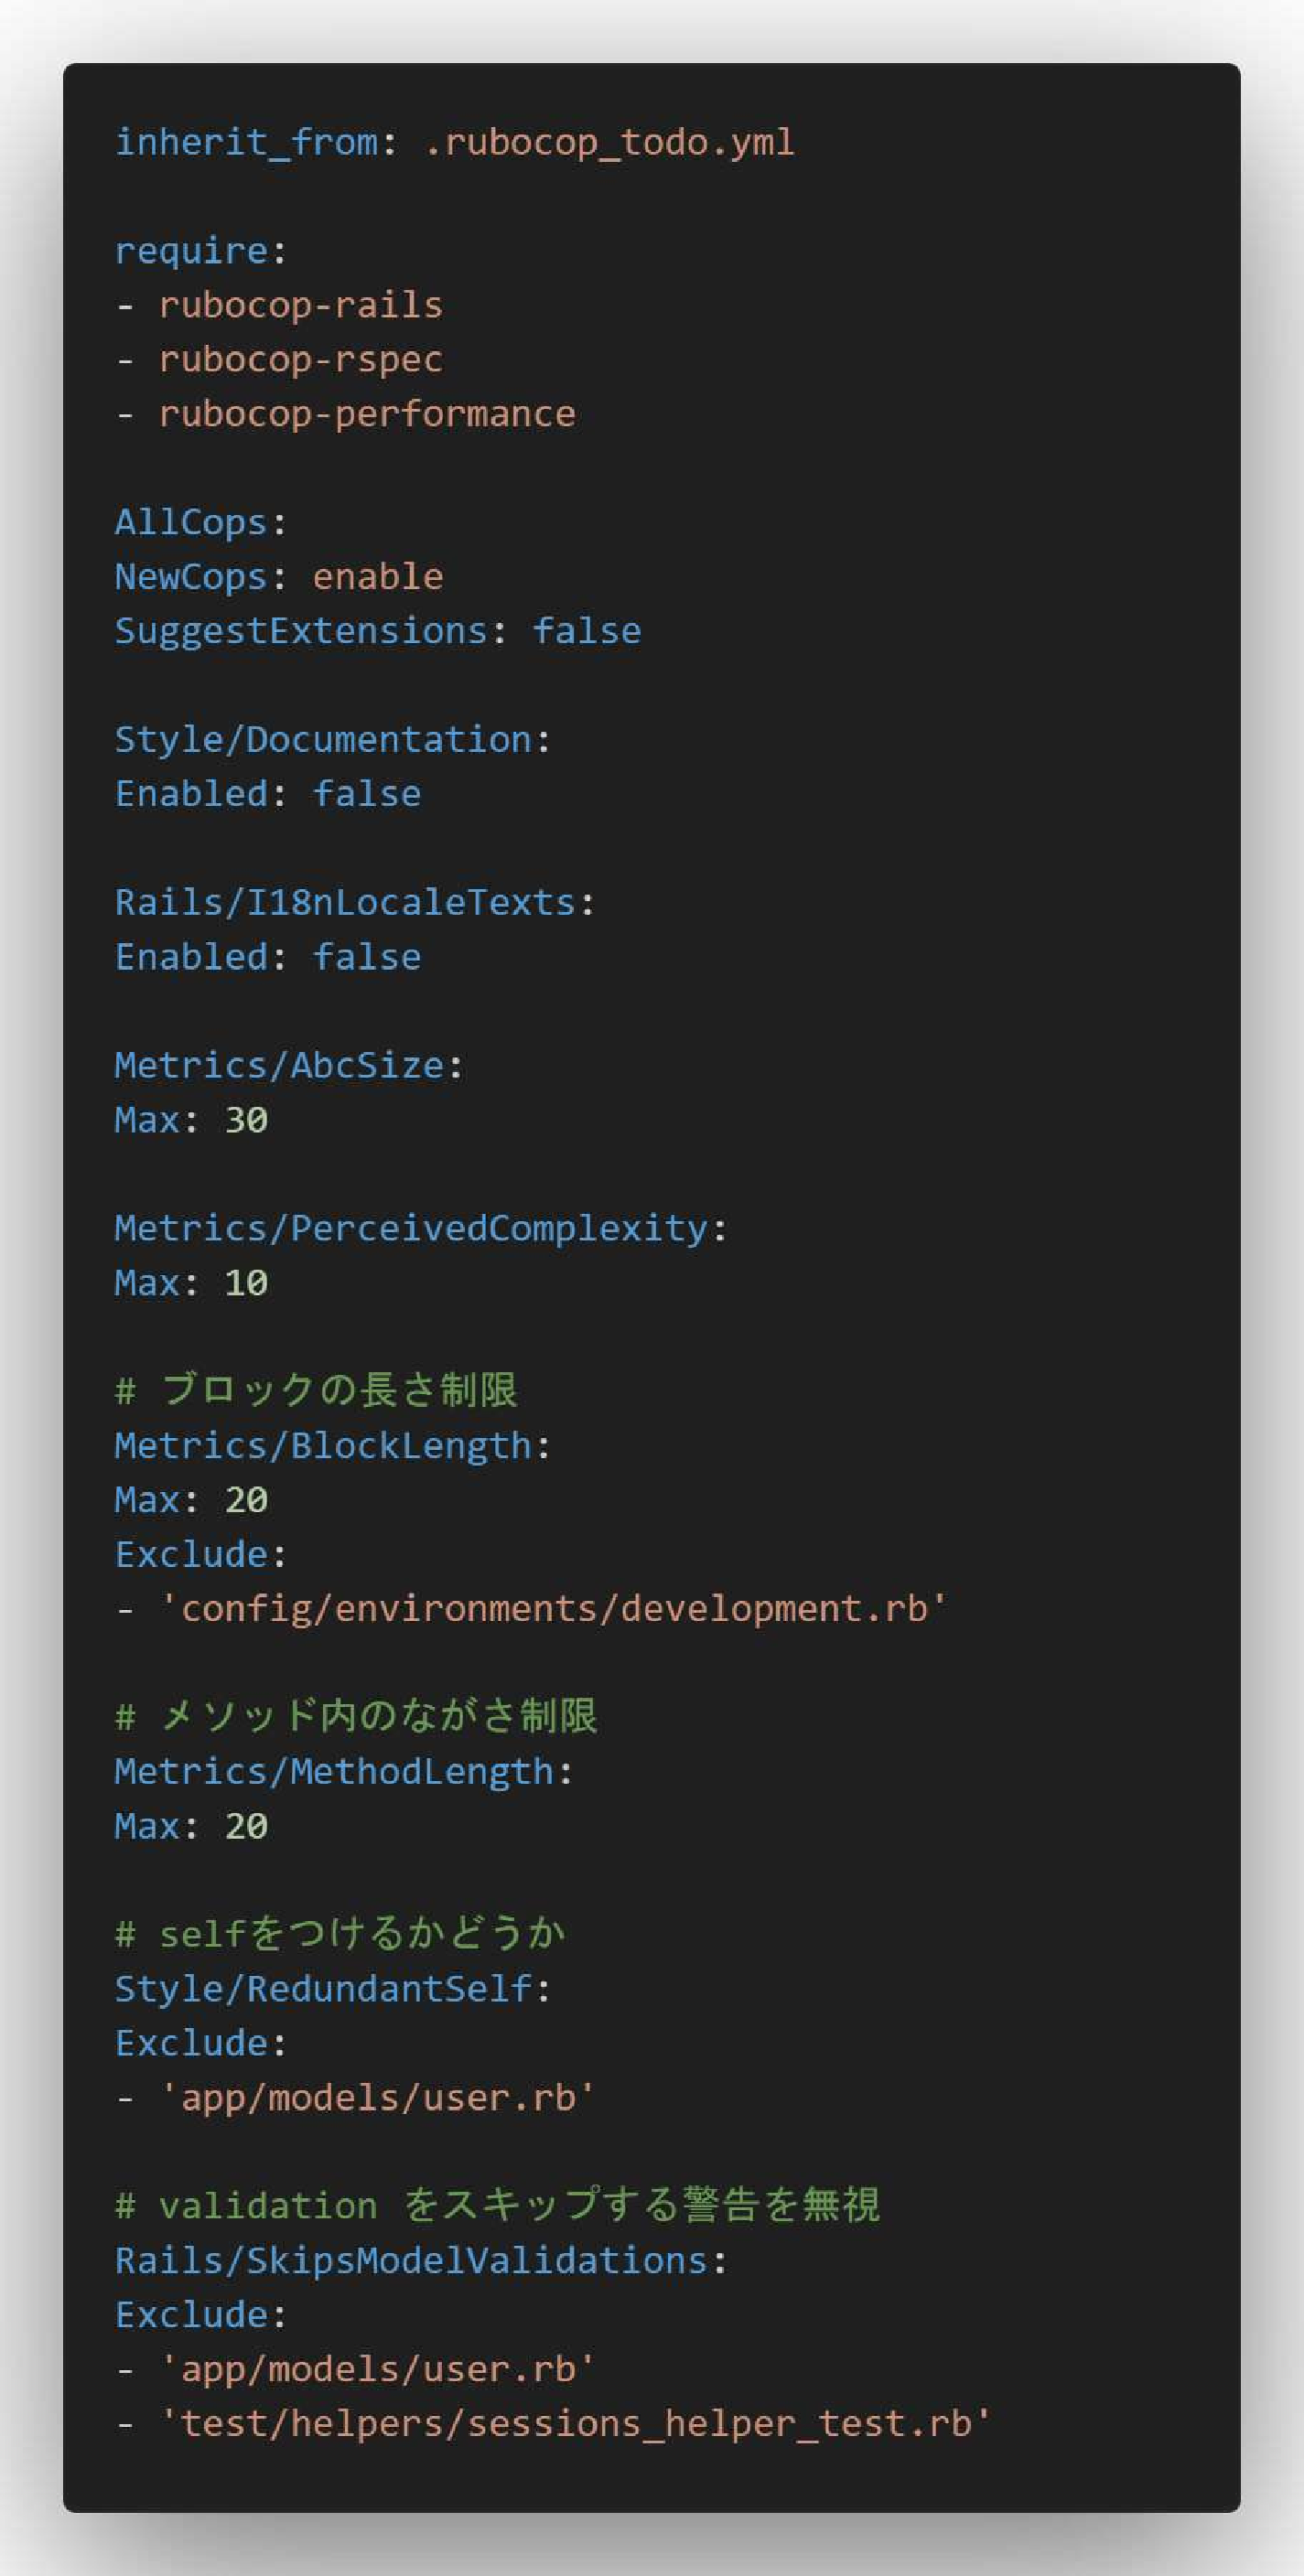
\includegraphics[scale=0.4]{img/etc/rubocop.pdf}
    \caption{rubocop設定ファイル}
    \label{rubocop}
\end{figure}

指摘された箇所は,全て確認,訂正する.
\newpage

\section{Railsフレームワーク規約}\label{q3.2}
Rails のフレームワークに従って実装する.RailsはMVCモデルを採用しているため,それぞれに命名はRailsが定める規則に従う.
\begin{itemize}
    \item Model
    \begin{enumerate}
        \item ファイル
        
        モデルファイルは,\texttt{app/model}ディレクトリ内に配置する.モデルファイル名は,\texttt{tableName.rb}とする.tableNameには作るデータテーブル名を単数形・小文字で書く.例えば,Userに関するデータテーブルを作りたい場合には,\texttt{user.rb}とする.
        
        \item クラス

        1つのファイルに,1つのクラスを記述する.クラス名は,ファイル名の先頭を大文字にしたものを使う.例えば,ファイル名が\texttt{user.rb}である場合,クラス名は\texttt{User}である.必ず,\texttt{ApplicationRecord}を継承する.
        
        \item マイグレーションファイル
        \begin{enumerate}
            \item[a.] ファイル
            
            マイグレーションファイルは,\texttt{db/migrate}ディレクトリ内に配置する.ファイル名は\texttt{timestamp\_verb.rb}とする.\texttt{verb}には動作を記入,ファイル名はスネークケースを用いて表現し,全て小文字とする.例えばUserデータベース内のEmail列にインデックスを追加するマイグレーションファイル名は,\texttt{timestamp\_add\_index\_to\_users\_email.rb}である.
            %\newpage
            \item[b.] クラス

            1つのファイルに,1つのクラスを記述する.クラス名は,ファイル名の\texttt{timestamp}と拡張子を除いてスネークケースで表現したものを用いる.上記の例に倣うと,クラス名は\texttt{AddIndexToUsersEmail}となる.
            
            必ず,\texttt{ActiveRecord::Migration[7.1]}を継承する.

            \item[c.] 関数名

            関数名は\texttt{change}とする.1つのクラスに1つの関数のみを定義する.
        \end{enumerate}
    \end{enumerate}
    
    \item Controller
    \begin{enumerate}
        \item ファイル

        コントローラファイルは\texttt{app/controllers}ディレクトリ内に配置する.コントローラのファイル名は,\texttt{viewContents\_controller.rb}とする.\texttt{viewContents}は表示したいものを複数形・小文字で書く.例えば,Userに関するコントローラの場合は,\texttt{users\_controller.rb}とする.
        \item クラス

        1つのファイルに,1つのクラスを記述する.クラス名はキャメルケースを用いて表現する.必ず,\texttt{ApplicationController}を継承する.例えば,
        
        \texttt{users\_controller.rb}内で定義されているクラス名は,\texttt{UsersController}である.
        \item アクション

        コントローラ内のアクション名は,全て小文字で表現する.原則,以下のアクション名を用いる.これ以外に定義する場合,全体で相談する.
        \begin{itemize}
            \item index
            \item home
            \item new
            \item create
            \item edit
            \item show
            \item update
            \item destroy
        \end{itemize}
    \end{enumerate}
    \item View
    \begin{enumerate}
        \item ファイル

        ビューファイルは,\texttt{app/view}ディレクトリ内に配置する.ディレクトリ内にサブディレクトリを”コントローラ名”で作り,その中に各アクションに対応するビューを作る.例えば,\texttt{users\_controller.rb}内で定義されたアクション\texttt{new}に対応するビューを作るなら,そのファイル名は\texttt{app/views/users/new.html.erb}となる.
    \end{enumerate}
\end{itemize}

\section{開発規約}\label{q3.3}
ソースコードの差分管理にはGitHubを用いる.差分ログをGitHub上へ反映することを「PUSH」と書く.また,CIをGitHub Actionsで実行する.内容は,\texttt{rubocop}と,\texttt{rails test}である.
\subsection{PUSHする前に}\label{q3.3.1}
PUSHする前に,テストを走らせ,rubocopを実行する.全て成功したらPUSHする.
\begin{screen}
    \texttt{\$ bundle exec rubocop}
    
    \texttt{\$ bundle exec rails test}
\end{screen}

\subsection{ブランチ}\label{q3.3.2}
\begin{itemize}
    \item メインブラインチを\texttt{develop}とする.
    
    \item \texttt{develop}ブランチへPUSHしないこと.必ずブランチを切って編集し,そのブランチ名でPUSHする.以下の項目が成功したら\texttt{develop}へマージする.
    \begin{enumerate}
        \item GitHub上でプルリクエストを作成する.
        \item CIが通っていることを確認する.
        \item 溝口洸熙がApproveする.
    \end{enumerate}
    
    \item ブランチ名は以下のように定める.
    \begin{itemize}
        \item[$\circ$] \texttt{docs/*}

        ドキュメントに関する更新
        \item[$\circ$] \texttt{fix/*}

        バグの更新
        \item[$\circ$] \texttt{future/*}

        新規機能の追加
    \end{itemize}
    
    \item 他ブランチ上で作業する時は,定期的に以下のコマンドを実行し,\texttt{develop}の更新を取り入れる.
    \begin{screen}
        \texttt{\$ git merge develop}
    \end{screen}
\end{itemize}

\subsection{タグ}\label{q3.3.3}
リリース作業にはgit Tagを用いる.タグの命名は以下のように行う.
\begin{screen}
    \texttt{v[major-Version].[minor-Version]}
\end{screen}

開始番号を\texttt{0}とし,バグ修正をminor-Version Up,新機能追加をmajor-Version Upとする.タグの更新をGitHub Actionsで検知し,AWSへオートデプロイ(CD)する.

